% Options for packages loaded elsewhere
\PassOptionsToPackage{unicode}{hyperref}
\PassOptionsToPackage{hyphens}{url}
%
\documentclass[
]{article}
\usepackage{amsmath,amssymb}
\usepackage{lmodern}
\usepackage{iftex}
\ifPDFTeX
  \usepackage[T1]{fontenc}
  \usepackage[utf8]{inputenc}
  \usepackage{textcomp} % provide euro and other symbols
\else % if luatex or xetex
  \usepackage{unicode-math}
  \defaultfontfeatures{Scale=MatchLowercase}
  \defaultfontfeatures[\rmfamily]{Ligatures=TeX,Scale=1}
\fi
% Use upquote if available, for straight quotes in verbatim environments
\IfFileExists{upquote.sty}{\usepackage{upquote}}{}
\IfFileExists{microtype.sty}{% use microtype if available
  \usepackage[]{microtype}
  \UseMicrotypeSet[protrusion]{basicmath} % disable protrusion for tt fonts
}{}
\makeatletter
\@ifundefined{KOMAClassName}{% if non-KOMA class
  \IfFileExists{parskip.sty}{%
    \usepackage{parskip}
  }{% else
    \setlength{\parindent}{0pt}
    \setlength{\parskip}{6pt plus 2pt minus 1pt}}
}{% if KOMA class
  \KOMAoptions{parskip=half}}
\makeatother
\usepackage{xcolor}
\IfFileExists{xurl.sty}{\usepackage{xurl}}{} % add URL line breaks if available
\IfFileExists{bookmark.sty}{\usepackage{bookmark}}{\usepackage{hyperref}}
\hypersetup{
  pdftitle={Introducción a las probabilidades (parte II)},
  hidelinks,
  pdfcreator={LaTeX via pandoc}}
\urlstyle{same} % disable monospaced font for URLs
\usepackage[margin=1in]{geometry}
\usepackage{color}
\usepackage{fancyvrb}
\newcommand{\VerbBar}{|}
\newcommand{\VERB}{\Verb[commandchars=\\\{\}]}
\DefineVerbatimEnvironment{Highlighting}{Verbatim}{commandchars=\\\{\}}
% Add ',fontsize=\small' for more characters per line
\usepackage{framed}
\definecolor{shadecolor}{RGB}{248,248,248}
\newenvironment{Shaded}{\begin{snugshade}}{\end{snugshade}}
\newcommand{\AlertTok}[1]{\textcolor[rgb]{0.94,0.16,0.16}{#1}}
\newcommand{\AnnotationTok}[1]{\textcolor[rgb]{0.56,0.35,0.01}{\textbf{\textit{#1}}}}
\newcommand{\AttributeTok}[1]{\textcolor[rgb]{0.77,0.63,0.00}{#1}}
\newcommand{\BaseNTok}[1]{\textcolor[rgb]{0.00,0.00,0.81}{#1}}
\newcommand{\BuiltInTok}[1]{#1}
\newcommand{\CharTok}[1]{\textcolor[rgb]{0.31,0.60,0.02}{#1}}
\newcommand{\CommentTok}[1]{\textcolor[rgb]{0.56,0.35,0.01}{\textit{#1}}}
\newcommand{\CommentVarTok}[1]{\textcolor[rgb]{0.56,0.35,0.01}{\textbf{\textit{#1}}}}
\newcommand{\ConstantTok}[1]{\textcolor[rgb]{0.00,0.00,0.00}{#1}}
\newcommand{\ControlFlowTok}[1]{\textcolor[rgb]{0.13,0.29,0.53}{\textbf{#1}}}
\newcommand{\DataTypeTok}[1]{\textcolor[rgb]{0.13,0.29,0.53}{#1}}
\newcommand{\DecValTok}[1]{\textcolor[rgb]{0.00,0.00,0.81}{#1}}
\newcommand{\DocumentationTok}[1]{\textcolor[rgb]{0.56,0.35,0.01}{\textbf{\textit{#1}}}}
\newcommand{\ErrorTok}[1]{\textcolor[rgb]{0.64,0.00,0.00}{\textbf{#1}}}
\newcommand{\ExtensionTok}[1]{#1}
\newcommand{\FloatTok}[1]{\textcolor[rgb]{0.00,0.00,0.81}{#1}}
\newcommand{\FunctionTok}[1]{\textcolor[rgb]{0.00,0.00,0.00}{#1}}
\newcommand{\ImportTok}[1]{#1}
\newcommand{\InformationTok}[1]{\textcolor[rgb]{0.56,0.35,0.01}{\textbf{\textit{#1}}}}
\newcommand{\KeywordTok}[1]{\textcolor[rgb]{0.13,0.29,0.53}{\textbf{#1}}}
\newcommand{\NormalTok}[1]{#1}
\newcommand{\OperatorTok}[1]{\textcolor[rgb]{0.81,0.36,0.00}{\textbf{#1}}}
\newcommand{\OtherTok}[1]{\textcolor[rgb]{0.56,0.35,0.01}{#1}}
\newcommand{\PreprocessorTok}[1]{\textcolor[rgb]{0.56,0.35,0.01}{\textit{#1}}}
\newcommand{\RegionMarkerTok}[1]{#1}
\newcommand{\SpecialCharTok}[1]{\textcolor[rgb]{0.00,0.00,0.00}{#1}}
\newcommand{\SpecialStringTok}[1]{\textcolor[rgb]{0.31,0.60,0.02}{#1}}
\newcommand{\StringTok}[1]{\textcolor[rgb]{0.31,0.60,0.02}{#1}}
\newcommand{\VariableTok}[1]{\textcolor[rgb]{0.00,0.00,0.00}{#1}}
\newcommand{\VerbatimStringTok}[1]{\textcolor[rgb]{0.31,0.60,0.02}{#1}}
\newcommand{\WarningTok}[1]{\textcolor[rgb]{0.56,0.35,0.01}{\textbf{\textit{#1}}}}
\usepackage{graphicx}
\makeatletter
\def\maxwidth{\ifdim\Gin@nat@width>\linewidth\linewidth\else\Gin@nat@width\fi}
\def\maxheight{\ifdim\Gin@nat@height>\textheight\textheight\else\Gin@nat@height\fi}
\makeatother
% Scale images if necessary, so that they will not overflow the page
% margins by default, and it is still possible to overwrite the defaults
% using explicit options in \includegraphics[width, height, ...]{}
\setkeys{Gin}{width=\maxwidth,height=\maxheight,keepaspectratio}
% Set default figure placement to htbp
\makeatletter
\def\fps@figure{htbp}
\makeatother
\setlength{\emergencystretch}{3em} % prevent overfull lines
\providecommand{\tightlist}{%
  \setlength{\itemsep}{0pt}\setlength{\parskip}{0pt}}
\setcounter{secnumdepth}{-\maxdimen} % remove section numbering
\ifLuaTeX
  \usepackage{selnolig}  % disable illegal ligatures
\fi

\title{Introducción a las probabilidades (parte II)}
\author{}
\date{\vspace{-2.5em}}

\begin{document}
\maketitle

{
\setcounter{tocdepth}{2}
\tableofcontents
}
\hypertarget{uniuxf3n-de-eventos}{%
\section{Unión de eventos}\label{uniuxf3n-de-eventos}}

{ a. Probabilidad de la Unión para eventos \textbf{\emph{NO}} mutuamente
excluyentes }

\(P(A \cup B) = P(A) + P(B) - P(A \cap B )\)

recordar que \$ P(A \cap B )\$ por que si se ve en un diagrama de Venn
existe una sección de que ambos ocurran como se ve en la siguiente
imagen :

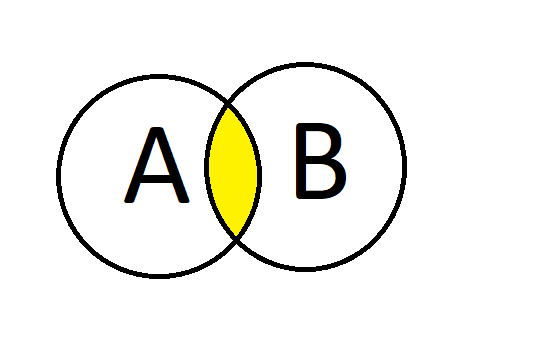
\includegraphics[width=3.125in,height=2.08333in]{ven_ex1.png}

{ b. Probabilidad de la Unión para eventos mutuamente excluyentes}

\(P(A \cup B) = P(A) + P(B)\)

En este caso sería un diagrama del siguiente estilo :

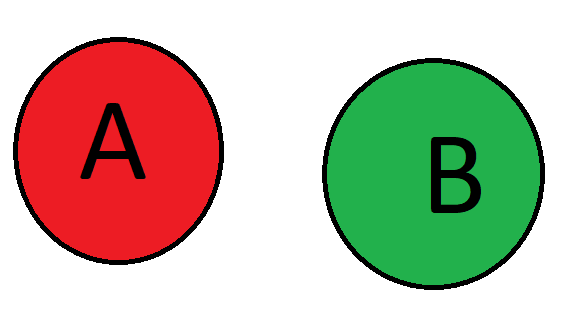
\includegraphics[width=3.125in,height=2.08333in]{venn_ex2.png}

{ b. Probabilidad de la Unión para tres eventos mutuamente excluyentes }

\(P(A \cup B \cup C ) = P(A) + P(B) + P(C) - P(A \cap B) - P(A\cap C ) - P(B \cap C) + P(A \cap B \cap C)\)
{ c.Probabilidad condicional }

\(P(A|B) = \frac{P(A \cap B)}{P(B)}\)

Esto se puede leer como ``Probabilidad de que ocurra A dado que ocurrió
B''

Ejemplo

En un curso de estadistica, la probabilidad de que un alumno estudie
materia es de un 75\% y la probabilidad de que practique código en R de
un 60\%. Además se sabe que la probabilidad de que estudie teoría y
practique código es de un 33\%. Entonces,¿Cuál es la probabilidad de que
practique código dado que estudio teoría?

\begin{Shaded}
\begin{Highlighting}[]
\CommentTok{\#Consideraremos A como  la probabilidad de que estudie teoría, y B que practique código}
\CommentTok{\#Y se quiere calcular la probabilidad de que ocurra B dado que ocurrio A. Osea}
\CommentTok{\#P(B|A) = P(A\^{}B) /P (A)}
\NormalTok{p\_A }\OtherTok{=} \FloatTok{0.75}
\NormalTok{p\_B }\OtherTok{=} \FloatTok{0.60}
\NormalTok{aYb }\OtherTok{=} \FloatTok{0.33}
\NormalTok{pCond }\OtherTok{=}\NormalTok{ aYb}\SpecialCharTok{/}\NormalTok{ p\_A}
\NormalTok{pCond}
\end{Highlighting}
\end{Shaded}

\begin{verbatim}
## [1] 0.44
\end{verbatim}

\hypertarget{intersecciuxf3n-de-eventos.}{%
\section{Intersección de eventos.}\label{intersecciuxf3n-de-eventos.}}

\hypertarget{reglas}{%
\subsection{Reglas}\label{reglas}}

{ Regla de la multiplicación }

\(P(A \cap B) = P(B|A) P(A) = \frac{P(A\cap B)}{P(A)} P(A)\)

o también

\(P(A \cap B) = P(A|B) P(B) = \frac{P(A\cap B)}{P(B)} P(B)\)

\hypertarget{independencia.}{%
\section{Independencia.}\label{independencia.}}

\hypertarget{introducciuxf3n-al-teoremas-de-bayes.}{%
\section{Introducción al Teoremas de
Bayes.}\label{introducciuxf3n-al-teoremas-de-bayes.}}

\hypertarget{bibliografuxeda}{%
\section{Bibliografía}\label{bibliografuxeda}}

{[}1{]} Montgomery, D. C., \& Runger, G. C. (2018). Applied statistics
and probability for engineers (7th ed.). Wiley.

\end{document}
